\section{Auswertung}
\label{sec:Auswertung}
Die in Abschnitt \autoref{sec:Auswertung} gezeigten Grafiken sind mithilfe der Python-Bibliotheken Matplotlib \cite{matplotlib}, Scipy \cite{scipy} und Numpy \cite{numpy}
erstellt worden.
\subsection{Magnetische Flussdichte einer langen und kurzen Spule in Abhängigkeit der Position auf der x-Achse}

Die aufgenommenen Messwerte für die kurze und lange Spule sind in \autoref{kurzeSpule} und \autoref{langeSpule} dargestellt.
\begin{figure}[H]
    \includegraphics[width=\linewidth]{build/kurzeSpule.pdf}
    \caption{Magnetische Flussdichte in Abhängigkeit der x-Position einer kurzen Spule.}
    \label{kurzeSpule}
\end{figure}
Die magnetische Flussdichte wird zum Mittelpunkt der kurzen Spule hin maximal und nimmt mit zunehmendem Abstand nach außen ab. 
Der Randpunkt der Spule ist in dem Graphen bei $x \approx \SI{4}{cm}$ zu lokalisieren. Hier ist eine Änderung des Abfalls zu erkennen.

\begin{figure}[H]
    \includegraphics[width=\linewidth]{build/langeSpule.pdf}
    \caption{Magnetische Flussdichte in Abhängigkeit der x-Position einer langen Spule.}
    \label{langeSpule}
\end{figure}
Bei der langen Spule zeigt sich ein ähnliches Verhalten. Die magnetische Flussdichte nimmt innerhalb der Spule nach außen hin ab. Am Randpunkt, hier bei 
$x \approx \SI{7}{cm}$ zu lokalisieren, ändert sich das Abnehmverhalten ebenfalls. Es flacht ab.
\\
\\
Bei beiden Spulen ist zu erkennen, dass an den Randpunkten ein Wendepunkt vorliegt. In dem Fall ist dort der stärkste Abfall der magnetischen
FFlussdichte zu beobachten.
\newpage
\subsection{Helmholtzspulenpaar}
Die Messwerte für die drei Konfigurationen sind in \autoref{helmholtz6}, \autoref{helmholtz12} und \autoref{helmholtz23} dargestellt.

\begin{figure}[H]
    \includegraphics[width=\linewidth]{build/helmholtz6.pdf}
    \caption{Magnetische Flussdichte in Abhängigkeit der x-Position eines Helmholtzspulenpaares mit Abstand $d =\SI{6}{cm}$.}
    \label{helmholtz6}
\end{figure}
Bei der Konfiguration $d = \SI{6}{cm}$ ist ein Abfall außerhalb des Spulenpaares zu erkennen.

\begin{figure}[H]
    \includegraphics[width=\linewidth]{build/helmholtz12.pdf}
    \caption{Magnetische Flussdichte in Abhängigkeit der x-Position eines Helmholtzspulenpaares mit Abstand $d =\SI{12}{cm}$.}
    \label{helmholtz12}
\end{figure}
Die Konfiguration mit $d = \SI{12}{cm}$ zeigt ein lokales Minimum in der Mitte des Spulenpaares bei $x \approx \SI{4}{cm}$. Weil die Spulen weiter auseinander sind
überlagern sich die Flussdichten der einzelnen Spulen nicht mehr stark genug, um ein Maximum in der Mitte des Spulenpaares zu erzeugen. Die magnetische Flussdichte ist also auch insgesamt schwächer im Vergleich zur Konfiguration mit $d = \SI{6}{cm}$ (vgl. \autoref{helmholtz6}).
Daraus resultieren dann auch die Maxima an den Rändern des Spulenpaares bei $x \approx \SI{0.5}{cm}$ und $x \approx \SI{6.5}{cm}$, da die Felder der einzelnen Spulen stärker als die Überlagerung in der Mitte sind. Außerhalb des Spulenpaares, also $d > \SI{12}{cm}$, fällt die 
magnetische Flussdichte ab.

\begin{figure}[H]
    \includegraphics[width=\linewidth]{build/helmholtz23.pdf}
    \caption{Magnetische Flussdichte in Abhängigkeit der x-Position eines Helmholtzspulenpaares mit Abstand $d =\SI{23.85}{cm}$.}
    \label{helmholtz23}
\end{figure}
Die Konfiguration mit $d = \SI{23.85}{cm}$ zeigt ebenfalls ein lokales Minimum in der Mitte des Spulenpaares bei $x \approx \SI{10}{cm}$. An den Rändern sind Maxima der magnetischen Flussdichte zu beobachten.
Dies beruht auf der gleichen Begründung wie bei der Konfiguration mit $d =\SI{12}{cm}$. Außerhalb scheint die Feldstärke wieder abzufallen.
\begin{figure}[H]
    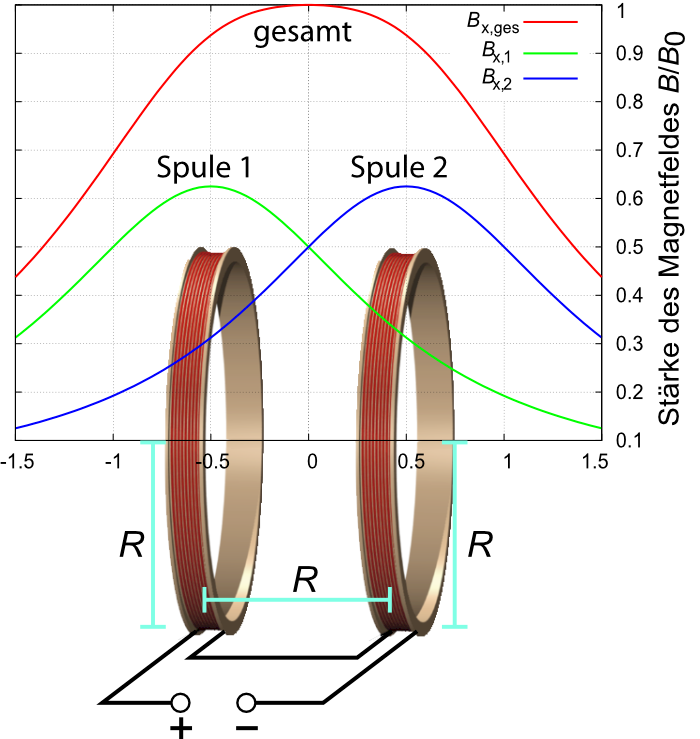
\includegraphics[width=\linewidth]{fotos/helmholtzspuletheriekurve.png}
    \caption{Aufbau und Theoriekurve der Helmholtz-Konfiguration mit $R = d$ \cite{leifi}.}
    \label{helmholtztheorie}
\end{figure}
Wie in \autoref{helmholtztheorie} zu sehen, überlagern sich die Felder der einzelnen Spulen in der Mitte. Im Vergleich mit \autoref{helmholtz12} und \autoref{helmholtz23}
ist zu sehen, dass für ein Maximum in der Mitte der Spulen der Abstand $d$ zwischen den Spulen nicht zu groß sein darf. Der Abfall außerhalb der Konfiguration stimmt
mit der Theorie überein.  
\newpage
\subsection{Hysteresekurve einer Spule mit Eisenkern}
In \autoref{hysterese} ist die Hysteresekurve einer Spule mit Eisenkern aufgetragen.
\begin{figure}[H]
    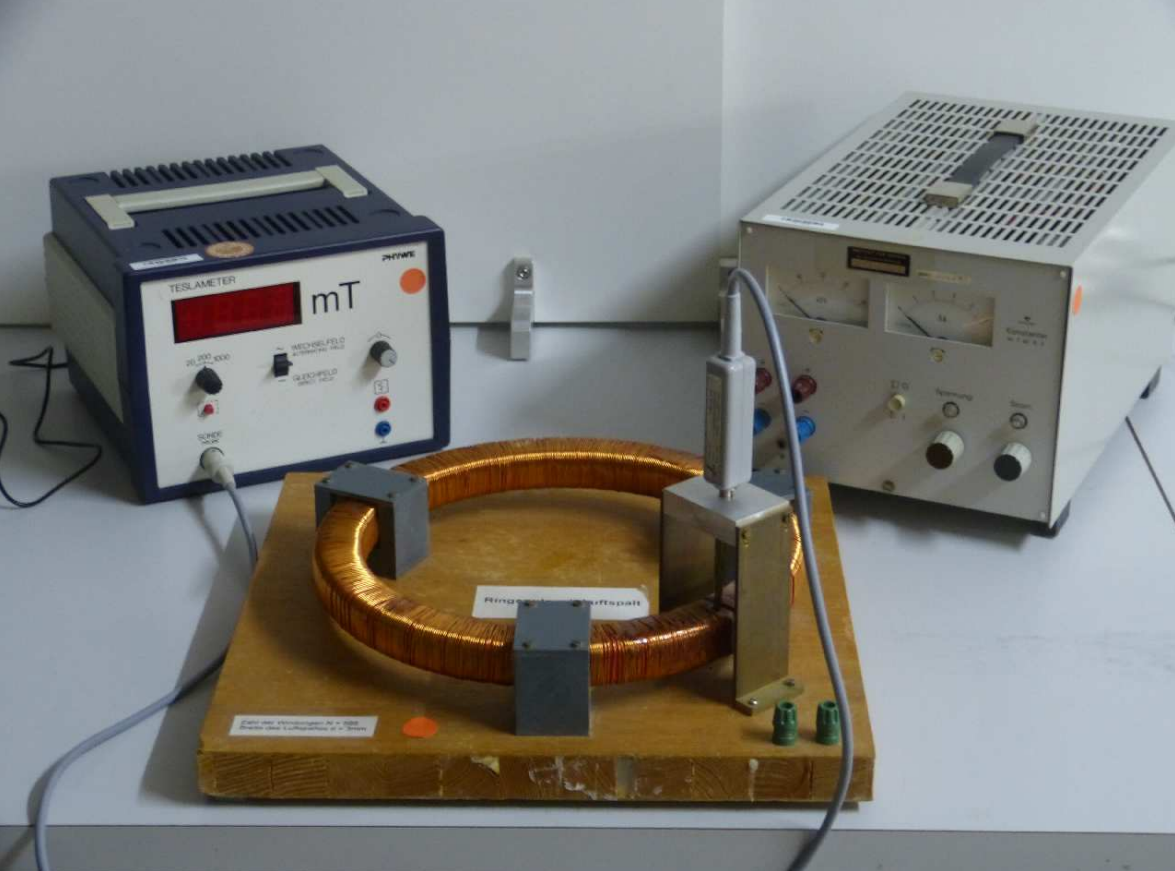
\includegraphics[width=\linewidth]{build/hysterese.pdf}
    \caption{$B$-$I$-Diagramm einer Spule mit Eisenkern.}
    \label{hysterese}
\end{figure}
Aus dieser lassen sich die Sättigungsmagnetisierung $B_S$, die Remanenz $B_r$ und
die Koerzitivkraft $H_c$ (da $H_c \propto I_c$) ablesen. Diese ergeben sich zu 
\begin{equation*}
    B_S = \SI{725}{mT},\;B_r = \SI{139}{mT} \text{ und } H_c = \SI{-350}{A/m}.
\end{equation*}
Dabei wurde der Zusammenhang 
\begin{equation*}
    H = I \cdot \frac{n}{2\pi r_T}
\end{equation*}
mit der Wicklungszahl $n = 595$, dem Spulenstrom $I$ und dem mittleren Spulenradius $r_T = \SI{0.135}{\meter}$ verwendet.
Die Funktion für die Neukurve wurde mit Polyfit \cite{scipy} an die Messwerte gefittet. Für die Fitfunktion wurde 
\begin{equation*}
    aH^5 + bH^4 + cH^3 + dH^2 + eH + f,
\end{equation*}
also ein Polynom fünften Grades, genutzt.
Die Koeffizienten ergeben sich zu
\begin{align*}
    a &= \SI{-3.708e-16}{[\milli\newton\m^4\per\A^6]},\\
    b &= \SI{6.822e-12}{[\milli\newton\m^3\per\A^5]},\\
    c &= \SI{-4.236e-08}{[\milli\newton\m^2\per\A^4]},\\
    d &= \SI{8.184e-05}{[\milli\newton\m\per\A^3]},\\
    e &= \SI{0.1553}{[\milli\newton\per\A^2]},\\
    \text{und }f &= \SI{4.428}{[\milli\newton\per\A\m]}.
\end{align*}
Um nach Gleichung \eqref{eq:diff} die differentielle Permeabilität der Neukurve zu bestimmen, muss die Fitfunktion nach $H$ abgeleitet und durch die Vakuum-Permeabilität 
geteilt werden. Dann ergibt sich:
\begin{align}\label{mudiff}
    \mu_{diff}(0)    &= \SI{123610}{[\milli\tesla\meter\per\ampere]} &= \SI{123.61}{[\tesla\meter\per\ampere]} &= 123.61 \\
    \mu_{diff}(\SI{7070}{\ampere\per\meter}) &= \SI{80280}{[\milli\tesla\meter\per\ampere]} &= \SI{80.28}{[\tesla\meter\per\ampere]} &= 80.28.
\end{align}













\newpage